\documentclass[11pt]{article}

\usepackage{exscale}
\usepackage{graphicx}
\usepackage{amsmath}
\usepackage{latexsym}
\usepackage{times,mathptm}
\usepackage{epsfig}
\usepackage{setspace}

\textwidth 6.5truein
\textheight 9.0truein
\oddsidemargin 0.0in
\topmargin -0.6in

\parindent 0pt
\parskip 5pt
\def\baselinestretch{1.1}

\begin{document}

\begin{LARGE}
\centerline {\bf CSci 423 Homework 11}
\end{LARGE}
\vskip 0.25cm

\centerline{Due: 1:00 pm, Wednesday, 11/28}
\centerline{Eric Shih}

\begin{enumerate}
  \item (10 points) Problem 5.17 on page 212. (Hint: Give a simple algorithm)
	If the alphabet is unary, the dominoes only differ in the number of $1s$ that each has on the top and bottom. This case is
	solved by:
	\begin{description}
	 \item M=“Given a collection of dominoes
	 \begin{enumerate}
	  \item If some domino has the same number of $1s$ on top and bottom, there is a trivial match, so accept.
	  \item If all the dominoes have more $1s$ on top than on bottom, there is no possibility of a match, so reject.
		Likewise, if all the dominoes have less 1’s on top than on bottom, reject.
	  \item Find one domino with more $1s$ on top than on bottom (say a difference of a $1s$), and one domino with more $1s$
		on bottom than on top (say a difference of b $1s$). Choosing b of the first domino and a of the second should make an
		an equal number of $1s$ on both top and bottom, and hence a match, thus accept.
	 \end{enumerate}
	\end{description}


  \item (10 points) This problem considers an attempt at a polynomial reduction from one problem to another that does not work.
	Your task is to find the flaw. A bipartite graph is an undirected graph in which every cycle has even length. We attempt
	to show that the Hamiltonian cycle (a cycle that passes through each node exactly once) problem polynomially reduces to the
	Hamiltonian cycle problem in bipartite graphs. We need a function $T$: \{graphs\}$\rightarrow$\{bipartite graphs\} such that
	T can be computed in polynomial time and for any graph $G$, $G$ has Hamiltonian cycle iff $T(G)$ has a Hamiltonian cycle.
	Let $T(G)$ be the bipartite graph obtained by inserting a new vertex on every edge. What is wrong with this transformation? \\

	This transformation has a condition that for any graph G, G has a Hamiltonian cycle iff T(T) has a Hamiltonian cycle. A
	counter-example will be used to show the error. If G is the graph shown here:
	\begin{center}
	  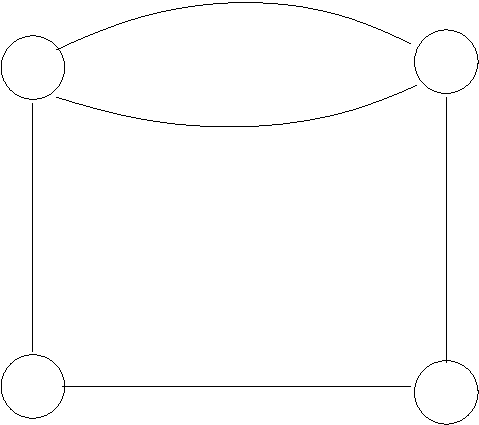
\includegraphics[scale=.4] {fig1.pdf} \\
	  Graph G
	\end{center}
	G does have a Hamiltonian cycle, but there is a T(G) that does not have a Hamiltonian path.
	\begin{center}
	  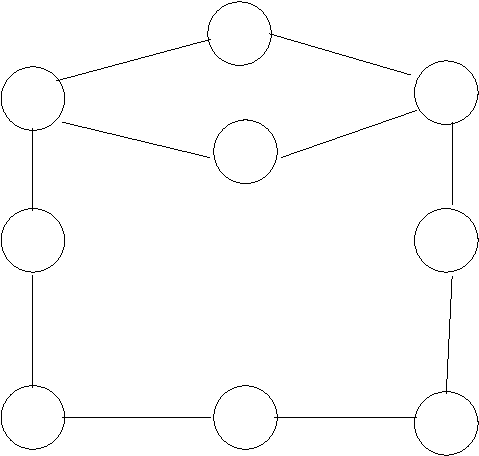
\includegraphics[scale=.4] {fig2.pdf} \\
	  Graph T(G)
	\end{center}
	From here, it is obvious that there is no path that visits each vertex once while also finishing at the starting vertex. Thus
	it does not have a Hamiltonian cycle showing what is wrong with the transformation.
  \item (10 points) The SET INTERSECTION (SI) problem is defined as follows: \\
	INSTANCE: Finite sets $A_1,\ldots,A_m$ and $B_1,\ldots,B_n$. \\
	QUESTION: Is there a set $T$ such that $|T\cap A_i|\ge 1$ for $i=1,\ldots,m$ and $|T\cap B_j|\le 1$ for $j=1,\ldots,n$? \\
	Show that SAT polynomially reduces to SI. \\
	*reference research.cs.queensu.ca/~cisc365/2010F/365$\%$20SetIntersectionNPC.pdf* \\

	For a CNF expression, $T$ can be transformed as follows:
	\begin{enumerate}
	 \item For each clause in the CNF expression, it is turned to set $A_i$. Each literal in $A_i$ becomes an element of the set. The unnegated
	 literal $x_i$ will become element $T_i$. Negated literal $\bar{x_i}$ will become element $F_i$. $m$ in the set intersection will equal the
	 number of clauses in the CNF expression
	 \item For each boolean variable, set $B_j$ can be created with elements $T_j$ and $F_j$. $n$ from the set intersection will be the
	 number of boolean variables.
	\end{enumerate}
	
\end{enumerate}

\pagebreak
\setlength{\parindent}{1cm}
\centerline{\bf Reading Summary 5}

\begin{spacing}{1.5}
 
\end{spacing}


\end{document}